\lstset{language=HTML}

\chapter{CouchApp}
\label{couchapp}
As already mentioned in Section~\ref{couchdb:restfulapi}, CouchDB also acts as web server, i.e. it provides resources (its documents), which are accessible via the web by using HTTP methods. Furthermore, CouchDB provides an integrated JavaScript web application framework called \emph{CouchApp}.\\
CouchApps are stored as common documents, or more precisely, \emph{design documents}. Hence, they are easy to edit and share, and are even replicable like other documents. However, this design documents have a lot of attachments, e.g. HTML and JavaScript files, images, CSS style sheets, etc.
\section{Developing CouchApps}
\label{couchapp:development}
To support the development and deployment of CouchApps, you can download and use the CouchApp tool\footnote{\url{http://couchapp.org}}. This tool prepares an appropriate CouchApp project structure on the one hand, and provides tool-supported deployment of the CouchApp on the other hand.\\
Moreover, we strongly recommend the use of a HTML and JavaScript editor providing syntax highlighting and auto completion, e.g. Microsoft's Visual Studio\footnote{\url{www.microsoft.com/visualstudio}}. For this purpose we created a CouchApp project template for Visual Studio 2012, which integrates the CouchApp tool and thus offers an Integrated Development Environment (IDE) for the development of CouchApps.\\
To deploy the project template in Visual Studio 2012, you just have to copy the template file "couch App.zip" into the project templates folder of Visual Studio (in windows operating systems: "<user>/Documents/Visual Studio 2012/Templates/ProjectTemplates). Consequently, in the "New Project" dialog of Visual Studio, the CouchApp template should appear, as shown in Figure~\ref{img:vsprojecttemplate}.
\begin{figure}[t!]
\centering
\includegraphics[width=0.75\columnwidth]{images/VSprojecttemplate.png}
\caption{CouchDB project template in Visual Studio}
\label{img:vsprojecttemplate}
\end{figure}
To ensure a faultless development of CouchApps with Visual Studio 2012, make sure to encode all files with UTF-8 (without signature) as shown in Figure~\ref{img:vsfileencoding}.

\begin{figure}[t!]
\centering
\includegraphics[width=0.50\columnwidth]{images/VSfileencoding.png}
\caption{Select "UTF-8 without signature" as encoding for all files in the CouchApp}
\label{img:vsfileencoding}
\end{figure}

A CouchApp project contains the following folders and files:
\begin{description}
\item[.couchappignore] Defines files or folders, which may be located inside the CouchApp directory, but should not be deployed to the CouchDB
\item[.couchapprc] May contain several deployment configurations, e.g. location of the CouchDB, authentication data, ...
\item[couchapp.json] Contains basic information about the CouchApp, e.g. its name, a short description, ...
\item[\_id] Contains the ID of the design document
\item[README.md] May provide some information about the CouchApp and how to access it
\item[\_attachments/] This folder contains the CouchApp's layout (index.html), CSS style sheets and some other files. These files will be deployed as attachments of the design document.
\item[vendor/] The files in this folder are usually from other sources, e.g. jQuery, jQuery UI, etc. These files will also be deployed as attachments of the design document.
\item[views/] May contain some predefined CouchDB views consisting of a map and an optional reduce function (as introduced in Section~\ref{couchdb:query}).
\end{description}
\section{Introduction to Evently}
\label{couchapp:evently}
Another very important folder in a CouchApp is "evently", which is containing folders and files belonging to the Evently jQuery plugin\footnote{\url{http://couchapp.org/page/evently}}. Evently empowers the developer to extend the set of common standard client-side web events (clicks, changes in text boxes, moving the mouse over a user control, ...) by more concrete custom events (selection of a specific device, submission of a new notification, ...).\\
Standard events are usually triggered by single elements of a browser's Document Object Model (DOM), e.g. a single button is clicked, the text in a text box has changed, the mouse enters the area of a div, a option in a drop-down list is selected, etc. These events can be handled by so-called event handlers, which are normally functions with the following two parameters:
\begin{description}
\item[sender] The sender parameter is the object, which triggered the event (e.g. the button which was clicked)
\item[args] This parameter may contain event-specific information (e.g. the selected option in a drop-down list)
\end{description}
\subsection{Evently Widgets}
\label{couchapp:evently:widgets}
While standard events are triggered by common DOM elements, Evently's custom events are triggered by so-called Evently \emph{widgets}. Initially, a widget is just an empty div, which will be filled by Evently with the widget's content, whereas each widget is represented by a folder in the "evently" directory of the CouchApp. The initial content of a widget is defined by the event handler for the "init" event of the widget, usually represented by the "\_init" subfolder in each widget's folder.\\
The communication between Evently widgets is done by custom events, i.e. one widget may trigger an event which is handled by another widget. For example, the following page (usually named "index.html" and located in the "\_attachments" folder of the CouchApp) contains two widgets "content" and "menu", whereas the "menu" widget provides the event "menuitemselected", which can be handled by the menu widget:
\begin{lstlisting}
<html>
  <head>
    <title>CouchApp</title>
  </head>
  <body>
    <div id="content"></div>
    <div id="menu"></div>
  </body>
  <script src="vendor/couchapp/loader.js"></script>
  <script type="text/javascript" charset="utf-8">
    $.couch.app(function (app) {
      $("#content").evently("content", app);
      $("#menu").evently("menu", app);

      $.evently.connect("#menu", "#content", ["menuitemselected"]);
    });
  </script>
</html>
\end{lstlisting}
Just like event handlers for the "init" event, event handlers for custom events are usually represented by subfolders of the corresponding widget folder. Therefore, concerning the example page from the listing above, the Evently folder contains the two widget folders "content" and "menu", whereas the "content" folder contains an event handler subfolder "menuitemselected". 

\subsection{Event handlers in Evently}
\label{couchapp:evently:eventhandlers}
An event handler in Evently define its widget's content, i.e. if an event is triggered by a widget A and handled by a widget B, the event handler replaces the current content of widget B. For this purpose, the event handler folder may contain the following components (files/subfolders), whereas each of them is optional:
\begin{description}
\item[data.js] Simply said, this file contains the actual event handler, i.e. it has to return data for the new content of the widget
\item[mustache.html] This file is a mustache\footnote{\url{http://mustache.github.io}} template, which may look like the following:
\begin{lstlisting}
<span>You have selected {{name}}</span>
\end{lstlisting}
These templates may contain certain tags (e.g. \{\{name\}\}), which are replaced by data returned from the function in data.js. For example, if the data function returns the object \emph{\{name : 'Option A'\}}, the template engine would generate the following markup:
\begin{lstlisting}
<span>You have selected Option A</span>
\end{lstlisting}
Moreover, mustache supports list tags, allowing the definition of templates for arrays:
\begin{lstlisting}
<ul>
    {{#people}}
  <li>{{lastname}}, {{firstname}}</li>
    {{/people}}
</ul>
\end{lstlisting}
Hence, if the data function returns the object \emph{\{people : [ \{lastname : 'Reschenhofer', firstname : 'Thomas'\}, \{lastname : 'Waltl', firstname : 'Bernhard'\} ]\}}, the template engine would generate the following markup:
\begin{lstlisting}
<ul>
  <li>Reschenhofer, Thomas</li>
  <li>Waltl, Bernhard</li>
</ul>
\end{lstlisting}

If the event handler does not contain a mustache template, the data function itself has to return well-formed markup.
\item[query.json] A common use case for event handlers is the query of data. For this purpose, the event handler may contain the file "query.json", which basically refers to a predefined or stored view in the CouchApp. The queried data is passed to the data function as parameter.
\item[async.js] Instead of using query.json and hence using a predefined query, an event handler may contain the file "async.js", which is often used to perform parametrized queries onto the database or to obtain data from other sources. Just like in query.json, the result of this function will be passed to the data function as parameter.
\item[after.js] The function in this file will be invoked after the generation of the widget's new content by the data function and the corresponding template. For example, the after function can be used to manipulate the generated content, or to perform certain loggings.
\item[selectors/] The selectors subfolder defines the behavior of the generated content. For example, a file "selectors/a/click.js" defines a event handler for the click event of each anchor in the generated content, whereas a file "selectors/a\#apply/click.js" affects only anchors with the id "apply".
\end{description}
Figure~\ref{img:eventlyeventhandler} illustrates the handling of events and the role of the listed components.\\
\begin{figure}[h!]
\centering
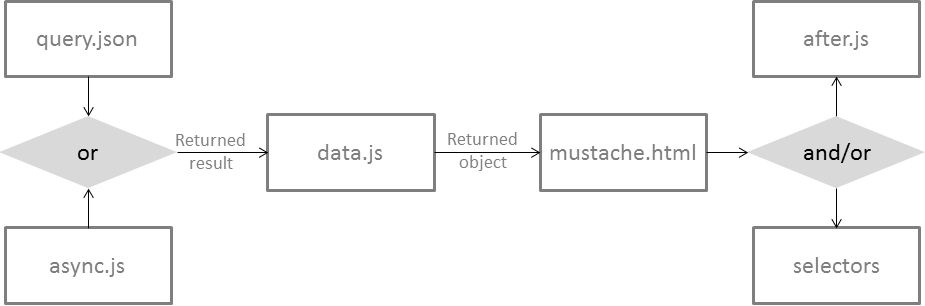
\includegraphics[width=1.00\columnwidth]{images/eventlyeventhandler.png}
\caption{Illustration of Evently's event handling}
\label{img:eventlyeventhandler}
\end{figure}
Actually, all the event handler's components need not to be defined in a certain folder structure, but can be defined in a single JSON file (i.e. all components are attributes of an event handler object). However, for the sake of clarity, the described approach is recommended.\\
Firing an event is done via a function provided by Evently. In the following example the \emph{this} keyword refers to the current widget (the "menu" from above), for which the event "menuitemselected" is triggered:
\begin{lstlisting}
$.couch.app(function (app) {
  $(this).trigger("menuitemselected");
});
\end{lstlisting}

\section{LabLOUNGE from a user's perspective}
\label{couchapp:labloungeuser}
To demonstrate the communication of a client with LabVIEW via CouchDB, we implemented a prototypical CouchApp named \emph{LabLOUNGE}\footnote{\url{https://github.com/treschenhofer/lablounge}}.\\
The LabLOUNGE page consist of three widgets:
\begin{description}
\item[main] The main content on the left side of the page, which shows either a device's data as time series (see Figure~\ref{img:lablounge01}), or a form for the submission of notifications to LabVIEW (see Figure~\ref{img:lablounge02}).
\begin{figure}[h!]
\centering
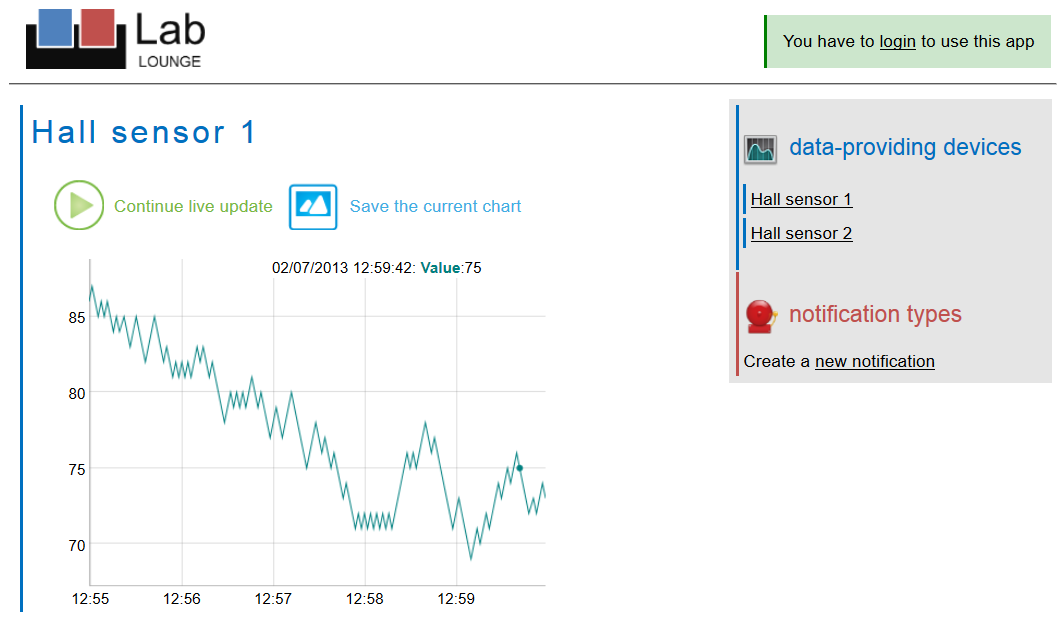
\includegraphics[width=1.0\columnwidth]{images/lablounge01.png}
\caption{The LabLOUNGE CouchApp in "plotting mode", showing a device's data as time series}
\label{img:lablounge01}
\end{figure}

\begin{figure}[h!]
\centering
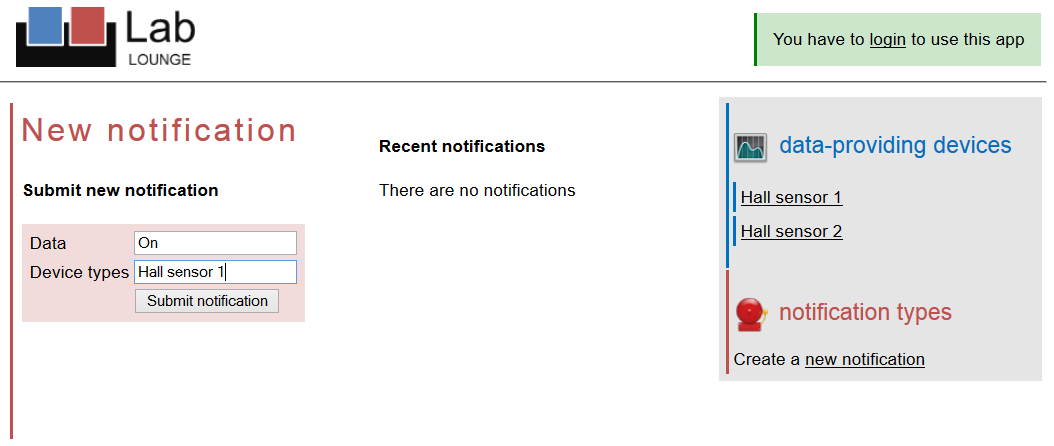
\includegraphics[width=1.0\columnwidth]{images/lablounge02.png}
\caption{The LabLOUNGE CouchApp in "notification mode", showing a form for the submission of notifications}
\label{img:lablounge02}
\end{figure}

\item[data-providing devices] A list of devices on the upper right side of the page, which contains all devices, for which there is at least one data entry in the database.

\item[notification types] A list of already submitted notifications grouped by their type on the lower right side of the page. Moreover, this widget contains a link to create a new notification.
\end{description}

\subsection{Time series}
As shown in Figure~\ref{img:lablounge01}, a device's data is represented as time series in a chart. This chart supports a live update feature, i.e. if a measuring device creates a permanent data stream, the changes feed of CouchDB can be used to respond to these changes by automatically updating the chart.\\
However, to save the chart as an image, the user can pause the live update to freeze the chart in order to open the chart as an image, which can be saved via the browser's "Save image as..." menu (see Figure~\ref{img:labloungechart}).\\
\begin{figure}[h!]
\centering
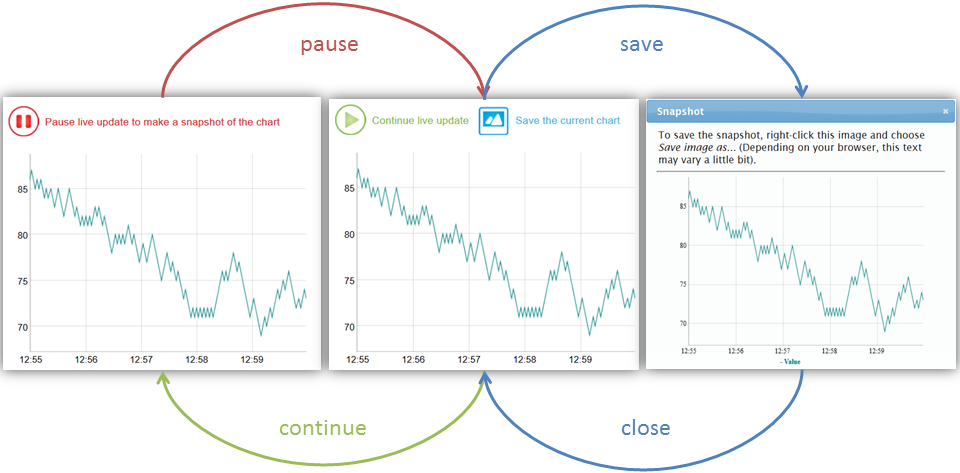
\includegraphics[width=1.0\columnwidth]{images/labloungechart.png}
\caption{A device's data plotted as a time series, which can be saved as an image}
\label{img:labloungechart}
\end{figure}
The live update can be reactivated at any time, s.t. each data set, which was created while the chart was frozen, is reloaded to update the chart.

\subsection{Notifications}
To send a notification via the CouchDB to LabLOUNGE, the user can either select an already existing notification type to resend a previously sent notification (see Figure~\ref{img:labloungenotification}), or create a new one.\\
\begin{figure}[h!]
\centering
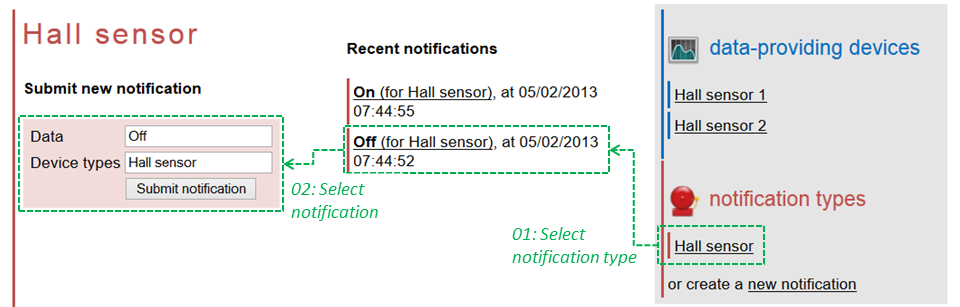
\includegraphics[width=1.0\columnwidth]{images/labloungenotification.png}
\caption{Creation of a new notification based on previously sent ones}
\label{img:labloungenotification}
\end{figure}

\section{LabLOUNGE from a developer's perspective}
\label{couchapp:labloungedeveloper}
The source project of our prototypical implementation can be found at GitHub\footnote{\url{https://github.com/treschenhofer/lablounge}} and opened with Visual Studio 2012. A CouchApp's structure and hence LabLOUNGE's project structure was already explained in Section~\ref{couchapp:development}.\\
As mentioned in the previous section, LabLOUNGE consists of three widgets: \emph{main}, \emph{devices}, and \emph{notificationtypes}. Their position on the page is defined in "index.html", which contains the associations of div elements with corresponding Evently widgets on the one hand, and the definition of widget connections on the other hand:
\begin{lstlisting}
$.couch.app(function (app) {
  $("#main").evently("main", app);
  $("#registereddevices").evently("devices", app);
  $("#notificationtypes").evently("notificationtypes", app);

  $.evently.connect("#registereddevices", "#main", 
		["deviceselected"]);
  $.evently.connect("#notificationtypes", "#main", 
		["notificationtypeselected"]);
});
\end{lstlisting}

\subsection{\emph{devices} widget}
\label{couchapp:labloungedeveloper:devices}
\begin{figure}[h!]
\centering
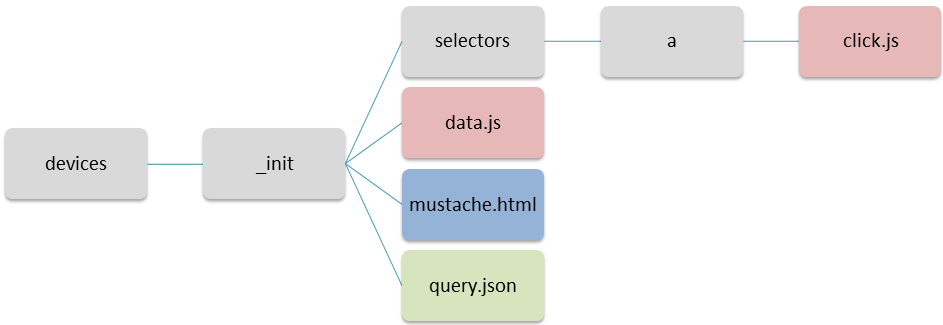
\includegraphics[width=1.0\columnwidth]{images/labloungestructuredevices.png}
\caption{Folder structure of the \emph{devices} widget}
\label{img:structuredevices}
\end{figure}
As shown in Figure~\ref{img:structuredevices}, this widget consists just of the "\_init" event handler. Therefore, when loading LabLOUNGE, this widget performs the query defined in "query.json", which is the predefined query "dataprovidingdevices" determining all devices providing at least one data entry.\\
The results are processed in data.js and forwarded to the mustache template, which generates a hyperlink (anchor) for each of the obtained devices. The selector defined in the widget applies to all of these anchors and handles their click events by storing the selected device onto the page and triggering the custom event "deviceselected", which will be handled by the \emph{main} widget (see Subsection~\ref{couchapp:labloungedeveloper:main}).

\subsection{\emph{notificationtypes} widget}
\label{couchapp:labloungedeveloper:notificationtypes}
\begin{figure}[h!]
\centering
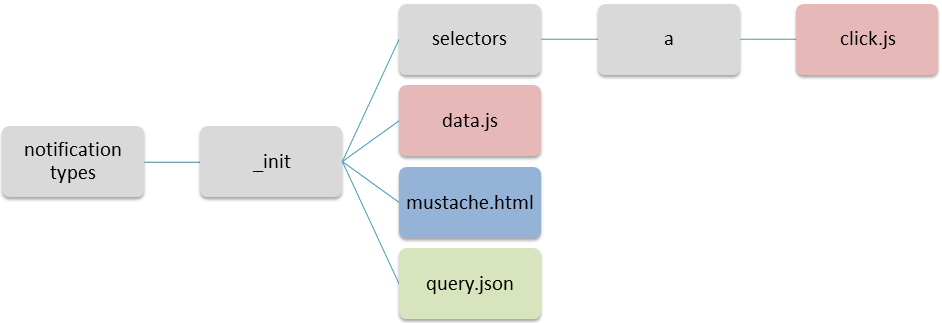
\includegraphics[width=1.0\columnwidth]{images/labloungestructurenotificationtypes.png}
\caption{Folder structure of the \emph{notificationtypes} widget}
\label{img:structurenotificationtypes}
\end{figure}
This widget's structure (depicted in Figure~\ref{img:structurenotificationtypes}) is very similar to the structure of the \emph{devices} widget. Again, there is just an "\_init" event handler, performing the predefined query "notificationtypes" when loading LabLOUNGE. This query determines all notification types, for which there is at least one notification instance.\\
Via the data function, these notification types are passed to the mustache template, which shows them as a list of anchors. Moreover, the template also defines a hyperlink for the creation of a new notification. Similar to the \emph{devices} widget, the selector in the \emph{notificationtypes} widget applies to all its anchors and handles the click events of them by storing the selected notification type onto the page and triggering the custom event "notificationtypeselected".
\subsection{\emph{main} widget}
\label{couchapp:labloungedeveloper:main}
\begin{figure}[h!]
\centering
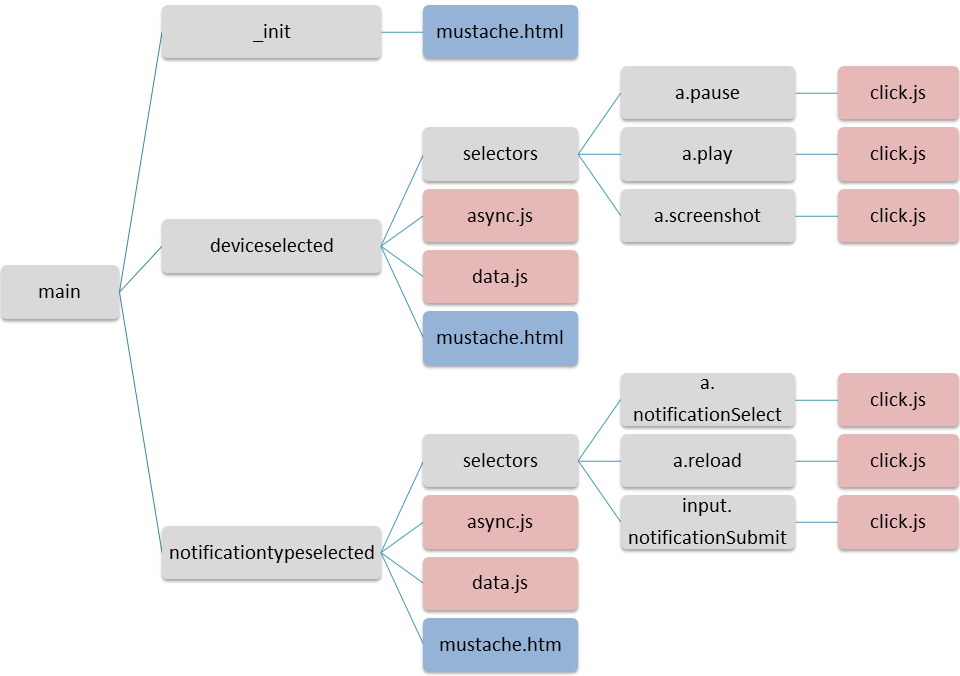
\includegraphics[width=1.0\columnwidth]{images/labloungestructuremain.png}
\caption{Folder structure of the \emph{main} widget}
\label{img:structuremain}
\end{figure}
As illustrated in Figure~\ref{img:structuremain}, the \emph{main} widget is the most complex one, since it consists of the three event handlers "\_init", "deviceselected", and "notifiationtypeselected".\\
The initial state of the \emph{main} widget is defined by the "\_init" event handler. However, since there is nothing to display before the selection of either a device or a notification type, this event handler consists only of a mustache template defining a simple static text.

\subsubsection{"deviceselected" event handler}
\label{couchapp:labloungedeveloper:main:deviceselected}
If the user selects a device in the \emph{devices} widget, the event "deviceselected" is triggered, which is handled by this event handler.\\
First, the async function determines the selected device and performs a query obtaining all the device's entries in reversed chronological order (the reversed order simplifies the adding of new entries by the live update feature). Furthermore, this function activates live update, i.e. LabLOUNGE will listen to the changes feed to immediately gather new created data entries.\\
After some processing of the obtained data in the data function, it is passed to the mustache template, where it is plotted as a time series, whereas plotting is done by the JavaScript Visualization library \emph{dygraphs}\footnote{\url{http://dygraphs.com}}. Moreover, the JavaScript library \emph{Moment.js}\footnote{\url{http://momentjs.com}} is used for the processing of datetime values.\\
The "deviceselected" event handler consists of three selectors:
\begin{description}
\item[a.pause] Handles the click event for the pause button. Stops the live update and showing buttons to continue the live update as well as to save the frozen chart.
\item[a.play] Handles the click event for the pause button. Continues the live update
\item[a.screenshot] Handles the click event for the save button. Opens a jQuery UI modal pop-up providing the frozen chart as a downloadable image.
\end{description}
The most interesting part of this widget is the live update feature, which is implemented in "\_attachments/logic.js".\\
On each change of the database's data this function is called, which is defined by the following lines of code:
\begin{lstlisting}
$dbname = "lablounge";
$appname = "labLounge";
$db = $.couch.db($dbname);
$db.changes().onChange(onDBChange);

function onDBChange(data) {
  ...
}
\end{lstlisting}
Since this function is invoked on EACH change of the database, it has to evaluate the relevance of the change for the live update feature by checking the following conditions:
\begin{itemize}
	\item Is currently any device selected at all, i.e. is LabLOUNGE in "plotting mode" (as in Figure~\ref{img:lablounge01}) or in "notification mode" (as in Figure~\ref{img:lablounge02})?
	\item Is live update activated or deactivated?
	\item Is the changed database document a data entry?
	\item And if yes, belongs this data entry to the selected device?
\end{itemize}

If the answer to all of these questions is "Yes", the new data entry is added to the plot.

\subsubsection{"notifiationtypeselected" event handler}
\label{couchapp:labloungedeveloper:main:notifiationtypeselected}
If the user selects a notification type in the \emph{notification type} widget, the event "notificationtypeselected" is triggered, which is handled by this event handler.\\
Similar to the "deviceselected" event handler, the async function first determines the selected notification type and performs a query obtaining all existing notification instances for the given type in reversed chronological order.\\
After some processing in the data function of this event handler, the obtained notifications are passed to the mustache template, which displays them as a list of anchors on the right side of the \emph{main} widget, and showing a form to submit a new notification on the left side of the \emph{widget} (see Figure~\ref{img:labloungenotification}).\\
The "a.notificationSelect" selector handles the click event of the anchors in the "Recent notifications" link by filling the form on the left side with the data of the chosen notification. The submission of a new notification is handled by the "input.notificationSubmit" selector, which creates a new notification object by the form data and saves this object as a document in the CouchDB:
\begin{lstlisting}
var notification =
{
  types : $("#deviceTypesDataField").val().split(","),
  data: $("#notificationDataField").val(),
  ...
};

$db.saveDoc(notification,
{
  success:function(data) {
    ...
  },
  error:function(ex){
    ...
  }
});
\end{lstlisting}